% !TEX TS-program = XeLaTeX+MakeIndex+BibTeX
% !TEX encoding = UTF-8 Unicode

\documentclass[12pt]{article}

%\usepackage[utf8]{inputenc}
\usepackage[brazilian]{babel}

\usepackage{fontspec}
\setmainfont{Linux Libertine G}
\linespread{1.05}

%%% PAGE DIMENSIONS
\usepackage{geometry} % to change the page dimensions
\geometry{a4paper} % or letterpaper (US) or a5paper or....
% \geometry{margin=2in} % for example, change the margins to 2 inches all round
% \geometry{landscape} % set up the page for landscape

\usepackage{graphicx} % support the \includegraphics command and options

% \usepackage[parfill]{parskip} % Activate to begin paragraphs with an empty line rather than an indent

%%% PACKAGES
\usepackage{amsfonts}
\usepackage{color}
%\usepackage{booktabs} % for much better looking tables
%\usepackage{array} % for better arrays (eg matrices) in maths
%\usepackage{paralist} % very flexible & customisable lists (eg. enumerate/itemize, etc.)
\usepackage{verbatim} % adds environment for commenting out blocks of text & for better verbatim
\usepackage{microtype}
\usepackage[numbers]{natbib}
%\usepackage{subfig} % make it possible to include more than one captioned figure/table in a single float
% These packages are all incorporated in the memoir class to one degree or another...

\usepackage[hidelinks]{hyperref}

% For Computer Modern:
%\def\Cpp{{C\nolinebreak[4]\hspace{-.05em}\raisebox{.4ex}{\tiny\bf ++}}}
% For Linux Libertine G
\def\Cpp{{C\nolinebreak[4]\raisebox{.20ex}{\small\bf++}}}

\newcommand{\todo}[1]{\textsf{\color{red}#1}}

%%% END Article customizations

\title{Exploração da Linguagem Rust para o Desenvolvimento de um Path Tracer Paralelo}
\author{Yuri Kunde Schlesner}
%\date{} % Activate to display a given date or no date (if empty), otherwise the current date is printed 

\begin{document}
\maketitle

\section{Identificação}

\begin{description}
	\item[Resumo:] \todo{TODO.}
	\item[Período de execução:] Setembro de 2014 a Dezembro de 2014
	\item[Unidades participantes:] ~\\ Curso de Ciência da Computação \\ Departamento de Eletrônica e Computação
	\item[Área de conhecimento:] Ciência da Computação
	\item[Linha de Pesquisa:] Computação Gráfica, Linguagens de Programação, Programação Paralela
	\item[Tipo de projeto:] Trabalho de Conclusão de Curso
	\item[Participantes:] ~\\ Profª Andrea Schwertner Charão -- Orientadora \\ Yuri Kunde Schlesner -- Orientando
\end{description}

\section{Introdução}

A \emph{Computação Gráfica} é a área da Ciência da Computação que estuda tópicos relacionados a
criação, análise e manipulação de imagens e conceitos relacionados. Dentre estas, a síntese (ou
renderização) de imagens é onde uma imagem é criada de forma computacional, a partir de um modelo
matemático e frequentemente buscando o fotorrealismo. Tem uma vasta quantidade de aplicações
práticas: É usada na engenharia, durante o projeto de máquinas ou construções; na arquitetura, para a
visualização de espaços; para entretenimento, em efeitos especiais de
filmes ou em jogos 3D e em muitas outras aplicações.

Como a geração de imagens fotorrealistas envolve essencialmente uma simulação completa da física da
luz, um processo proibitivamente lento e complexo, são utilizadas simplificações e modelos. No
passado, devido a limitada capacidade computacional disponível, eram utilizadas aproximações
grosseiras que, embora produzissem imagens atrativas, não eram muito realísticas, especialmente no
quesito da aparência das superfícies de suas interações com a luz. Com o aumento do poder
computacional disponível, vem sendo usados modelos mais fiéis a realidade e que produzem
imagens mais convincentes, algumas vezes indistinguíveis de uma fotografia real.

\emph{Path tracing} é um método de renderização que assume que a luz se comporta como uma partícula
e calcula uma imagem traçando uma série de raios pelos caminhos através quais a luz viajaria quando
refletida através de uma cena. Atualmente é um dos algoritmos mais usados quando são demandadas
imagens com um grau de realismo extremamente alto, devido a sua habilidade de simular o comportamento
da luz com relativa precisão.

No entanto, este realismo vem ao custo de muito poder de processamento, e mesmo com o avanço
tecnológico de CPUs, a renderização de imagens continua sendo uma das tarefas mais árduas para
processadores. Sistemas de renderização profissionais são quase exclusivamente escritos em \Cpp, e
não em linguagens de mais alto nível, devido as penalidades de performance que impõem. Sistemas
mais recentes chegam a fazer o uso de GPUs para acelerar a imensa quantidade de cálculos necessária.
Tendo em vista a baixa expressividade de \Cpp\ comparada a estas outras linguagens, torna-se
interessante explorar alternativas que permitam mais fácil desenvolvimento mas sem sacrificar a
performance requerida.

A linguagem de programação \emph{Rust}, um projeto de pesquisa da \emph{Mozilla Research}, tem como
seu objetivo ser uma união entre linguagens de programação de sistemas e as tidas como ``linguagens
de alto-nível'', focando simultaneamente em alta-performance, segurança e expressividade. Ela atinge
isso usando um modelo tradicional de compilação prévia (\emph{ahead of time}) e um sistema de tipos
que permite a verificação automática dos usos de ponteiros durante a compilação, eliminando a
possibilidade de acontecerem erros de memória sem introduzir penalidades excessivas de
performance ou consumo de memória. Ao mesmo tempo, integra conceitos mais recentes de linguagens
de programação que aumentam sua expressividade e capacidade de facilmente descrever programas
complexos.

\section{Objetivos}

\subsection{Objetivo Geral}

O objetivo geral deste trabalho é portar um \emph{path tracer} para Rust e, através deste processo,
realizar uma comparação qualitativa e quantitativa entre esta linguagem e \Cpp, nos aspectos de
performance e organização de código. Como base será utilizado o
SmallVCM\citep{smallvcm}, um path tracer de propósito educativo escrito em
\Cpp, escolhido por implementar uma variedade de algoritmos diferentes de path tracing e por ser
relativamente compacto, consistindo de aproximadamente 5000 linhas de código.

\subsection{Objetivos Específicos}
\begin{itemize}
	\item Estudar o código original do SmallVCM.
	\item Re-escrever um subconjunto mínimo do SmallVCM utilizando Rust, para a realização de
		testes.
	\item Realizar uma comparação de performance e clareza de código entre as duas versões e
		identificar possíveis melhorias.
	\item Paralelizar o renderizador, afim de melhorar sua performance, fazendo uso das
		funcionalidades de Rust.
	\item Portar o restante do SmallVCM, afim de que as duas versões tenham funcionalidades
		equivalentes.
\end{itemize}

\section{Justificativa}

Rust é uma linguagem relativamente nova e, embora aplicações gráficas de alta performance sejam um
dos seus públicos alvo, ainda não existe uma quantidade significativa de programas deste tipo que
valide a linguagem para este propósito. A experiência e resultados adquiridos durante a realização
deste trabalho podem ajudar a guiar o desenvolvimento da linguagem para atingir este fim.

\section{Revisão de Literatura}

\subsection{Path Tracing}

\emph{Path tracing} faz parte de uma família de algoritmos comumente denominados algoritmos de
\emph{ray tracing}. Embora também utilizados na física e nas engenharias, no contexto deste trabalho
são algoritmos que tem como finalidade a produção de imagens que retratam cenas tridimensionais.

Todos os algoritmos desta família se baseiam na ideia fundamental de simular o comportamento da luz
traçando raios que saem da câmera virtual em direção a cena. Isto é o contrário do que ocorre na
vida real, onde a luz é emitida de uma fonte e viaja pelo espaço até chegar ao observador, mas não
afeta negativamente o resultado final e torna o algoritmo computacionalmente viável, pois assegura
que todo o raio traçado é um que eventualmente chegaria no observador. (A maioria da
luz numa cena não chega até o observador, que subtende um espaço relativamente pequeno nela.)\citep{pharr2010}

Os primeiros algoritmos deste tipo a serem usados simplesmente traçavam um raio por pixel da imagem,
encontrando a intersecção deste raio com a cena e calculando sua aparência de acordo com algum
modelo básico de iluminação. Desta forma, não eram reproduzidas sombras nem superfícies refletivas, como
espelhos ou objetos metálicos. Estes tipo de algoritmos vieram a ser chamado de algoritmos de
\emph{ray casting}.

\Citet{whitted1980} propôs um novo método que soluciona estes problemas. Além do primeiro raio
partindo da câmera, são também traçados raios que vão do ponto sendo iluminado até cada uma das
fontes luminosas, permitindo que cada luz só seja adicionada se não estiver obstruída por outro
objeto e assim permitindo a renderização de sombras. Em superfícies refletivas, outro raio é traçado
na direção do reflexo, o qual é utilizado para calcular a luminosidade naquela direção, da mesma
maneira que o raio inicial. Assim, este algoritmo implementa \emph{ray tracing recursivo}.

\Citet{cook1984} aprimoraram o algoritmo de \citeauthor{whitted1980} para que suporte uma variedade
de efeitos adicionais como superfícies foscas e translúcidas, sombras com penumbras realísticas,
profundidade de campo e borrão de movimento. Todos estes efeitos são realizados através do mesmo
método de tirar várias amostras em cada ponto da imagem, introduzindo uma variação nas direções ou
posições traçadas em cada amostra. Embora não tenha o embasamento matemático, esta é a mesma ideia
básica utilizada posteriormente em algoritmos que utilizam integração Monte Carlo.

\Citet{kajiya1986} introduz a \emph{equação de renderização}, que descreve a interação da luz com as
superfícies, modelando também a reflexão de luz em superfícies completamente foscas (ver
\autoref{fig:path_tracing}.) Esta serve como uma importante fundação teórica que é usada como base
para o cálculo da imagem ou para o desenvolvimento de aproximações. No mesmo artigo é introduzida a
técnica de \emph{path tracing}, que difere das anteriores desenvolvidas por \citeauthor{cook1984} e
\citeauthor{whitted1980} por observar que os raios mais impactantes na aparência final da imagem são
os de baixa profundidade, e assim traçando apenas um raio recursivo por amostra, evitando o
crescimento exponencial do número de raios traçados que ocorre com as outras técnicas.

Embora capaz de produzir imagens extremamente realísticas, \emph{path tracing} pode requerer uma
quantidade impraticável de amostras para renderizar satisfatoriamente certos tipos de cenas onde não
exista uma linha de visão direta entre as superfícies e as fontes de luz. Nestas cenas a maioria da
iluminação se dá através de caminhos indiretos ou através de superfícies refratantes que projetem
padrões de luz complicados em outras superfícies (conhecidos como \emph{caustics}). Para contornar
estes problemas foram desenvolvidas inúmeras extensões ao algoritmo de path tracing. Dentre elas se
destaca \emph{bidirectional path tracing}, introduzido por \citet{lafortune1993}. Este algoritmo foi
depois reformulado por \citeauthor{veach1997} em \citep{veach1997}, onde também introduz a técnica
de \emph{multiple importance sampling} e o algoritmo \emph{Metropolis light transport}.

\begin{figure}
	\centering
	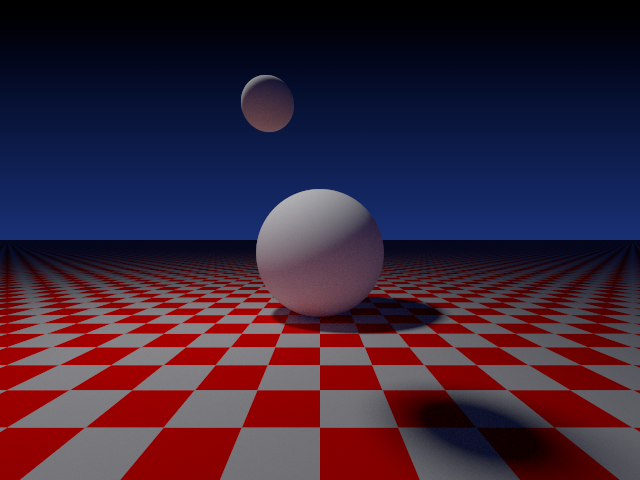
\includegraphics[width=0.5\textwidth]{exemplo_imagem}
	\caption{
		Um exemplo de uma imagem gerada utilizando \emph{path tracing}. Note como a luz que atinge o
		plano xadrez é refletida de volta para iluminar a esfera, um fenômeno conhecido como
		\emph{iluminação indireta} e que é corretamente simulado pelo algoritmo.
	}
	\label{fig:path_tracing}
\end{figure}

\subsection{Rust}

\todo{TODO}

\section{Metodologia}

Dado seu caráter prático, de implementar um programa em uma nova linguagem, esta pesquisa se
enquadra como pesquisa aplicada. Como o objetivo será de explorar melhores práticas e as possíveis
vantagens conferidas pela linguagem durante este processo, é uma pesquisa exploratória.

\section{Plano de Atividades e Cronograma}

\begin{enumerate}
	\item \label{activity:study} \textbf{Estudar o código original do SmallVCM:}
		Será feito um estudo do SmallVCM original, afim de aprender como é organizado e como pode
		ser melhor expresso em Rust.
	\item \label{activity:initial_port} \textbf{Re-escrever um subconjunto mínimo do SmallVCM utilizando Rust:}
		Para economizar tempo nesta etapa, serão portados apenas os algoritmos essenciais
		necessários para a renderização de imagens. O restante do programa será portado depois
		durante a etapa \ref{activity:finish_port}.
	\item \label{activity:compare} \textbf{Realizar uma comparação entre as duas versões:}
		As duas versões do renderizador, a nova feita em Rust e a antiga em \Cpp, serão comparadas
		nos quesitos de performance e de organização do código, afim de identificar avanços ou
		regressos, e se esses podem ser atribuídos a características de cada linguagem.
	\item \label{activity:parallelize} \textbf{Paralelizar o renderizador:}
		A nova versão do renderizador será paralelizada, afim de fazer melhor uso do hardware. Para
		atingir este objetivo serão exploradas todas as alternativas oferecidas pela linguagem, não
		se limitando a um tipo específico de paralelização.
	\item \label{activity:finish_port} \textbf{Portar o restante do SmallVCM:}
		O trabalho iniciado na etapa \ref{activity:initial_port} será finalizado com a escrita do
		restante do SmallVCM, afim de que a versão em Rust implemente a mesmas funcionalidades que a
		original. De acordo com a disponibilidade de tempo, este código novo também sera
		paralelizado.
\end{enumerate}

Espera-se que o desenvolvimento das atividades siga o seguinte cronograma:

\begin{table}[ht]
\centering
\begin{tabular}{c|cccc}
	Etapa & Setembro & Outubro & Novembro & Dezembro \\ \hline
	\ref{activity:study} & \checkmark & & & \\
	\ref{activity:initial_port} & \checkmark & \checkmark & & \\
	\ref{activity:compare} & & \checkmark & & \checkmark \\
	\ref{activity:parallelize} & & \checkmark & \checkmark & \checkmark \\
	\ref{activity:finish_port} & & & \checkmark & \checkmark \\
\end{tabular}
\caption{Cronograma de Atividades}
\end{table}

\section{Recursos}

Para a realização deste trabalho será utilizado apenas equipamento pessoal do pesquisador, visto que
não é necessário o uso de qualquer equipamento especial além de um computador para desenvolvimento.

\section{Resultados Esperados}

Ao término deste trabalho, espera-se ter uma implementação de um renderizador, escrito em Rust, que
seja capaz de produzir imagens fotorrealistas, fazendo uso eficiente do paralelismo oferecido pelo
hardware.

\bibliographystyle{abbrvnat}
\bibliography{../graphics}

\end{document}
